% Final project report -- NIT Warangal, M.Tech CSE
% Compile: pdflatex main.tex (twice)  |  or: tectonic main.tex  |  or upload the folder to Overleaf
\documentclass[11pt,a4paper]{article}

\usepackage[T1]{fontenc}
\usepackage[utf8]{inputenc}
\usepackage{newtxtext,newtxmath}
\usepackage[a4paper,margin=2.2cm,headheight=14pt]{geometry}
\usepackage{graphicx}
\usepackage{booktabs}
\usepackage{tabularx}
\usepackage{array}
\usepackage{multirow}
\usepackage{amsmath}
\usepackage{float}
\usepackage{caption}
\usepackage{subcaption}
\usepackage{enumitem}
\usepackage{xcolor}
\usepackage{fancyhdr}
\usepackage{algorithm}
\usepackage{algpseudocode}
% hyperref omitted: the Tectonic 0.15 build used to compile this PDF fails on it.
% For pdflatex or Overleaf you may add: \usepackage[hidelinks]{hyperref}

\graphicspath{{figures/}}
\captionsetup{font=small,labelfont=bf}
\setlist{itemsep=2pt,topsep=4pt}
\renewcommand{\arraystretch}{1.15}
\setlength{\emergencystretch}{1.5em}
\newcolumntype{Y}{>{\raggedright\arraybackslash}X}

\pagestyle{fancy}
\fancyhf{}
\fancyhead[L]{\small NIT Warangal}
\fancyhead[R]{\small Imagined-Shape EEG Classification}
\fancyfoot[C]{\small\thepage}
\renewcommand{\headrulewidth}{0.4pt}

\newcommand{\ga}{GA-NSGA}
\newcommand{\gas}{GA single-obj.}
\newcommand{\fb}{FBCSP-all}

\begin{document}

% ------------------------------------------------------------------ cover
\begin{titlepage}
\centering
\vspace*{1.2cm}

\includegraphics[width=3.2cm]{nitw_logo.png}\par
\vspace{0.8cm}
{\large\bfseries NATIONAL INSTITUTE OF TECHNOLOGY, WARANGAL\par}
\vspace{0.15cm}
{\normalsize Warangal, Telangana, India\par}
\vspace{1.0cm}
{\large\bfseries PROJECT REPORT\par}
\vspace{0.8cm}
{\LARGE\bfseries Classifying imagined shapes\\[0.2cm]
(circle/square/pentagram) from EEG signals\par}
\vspace{0.4cm}
{\normalsize Stability-aware selection of channels, frequency bands and time windows\\
Final Report\par}
\vspace{1.0cm}
{\normalsize Master of Technology\\
Department of Computer Science and Engineering\par}
\vspace{1.0cm}
{\normalsize\bfseries Submitted by\par}
\vspace{0.4cm}
{\normalsize\bfseries Abhay Nagesh Rao\par}
{\normalsize Roll No.: 26CSM1R01\par}
\vspace{0.3cm}
{\normalsize\bfseries Pandya Aditya Deepakkumar\par}
{\normalsize Roll No.: 26CSM1R02\par}
\vspace{0.3cm}
{\normalsize\bfseries Mulakalapalli Jayachandra Siddhartha\par}
{\normalsize Roll No.: 26CSM1R07\par}
\vfill
{\normalsize National Institute of Technology Warangal\par}
\end{titlepage}

% ------------------------------------------------------------------ abstract
\section*{Abstract}
Electroencephalography (EEG)-based visual-imagery brain--computer interfaces try to infer the
shape a person is imagining from their brain activity. We tested whether a \emph{stability-aware
multi-objective genetic algorithm} (NSGA-II) that jointly selects EEG channels, frequency bands and
time windows for a filter-bank common-spatial-pattern (FBCSP) and shrinkage-LDA classifier decodes
imagined shapes better than the same classifier on all components. We used the public visual-imagery
dataset of Gao et al.\ (22 participants, 42 sessions; circle, square and pentagram; chance $=1/3$)
under a strict protocol: leave-one-block-out and cross-session evaluation, with every selection nested
inside the training data and a hypothesis pre-registered before the results were analysed.
\textbf{The primary hypothesis is not supported:} the GA reached a balanced accuracy of 0.345 against
0.353 for the full baseline ($\Delta=-0.007$, one-sided Wilcoxon $p=0.79$, $n=22$). No pre-registered
secondary comparison was significant: an accuracy-only GA, cross-session evaluation, and EEGNet with 32
or 8 channels all gave Holm-corrected $p=1.00$. The GA matched the baseline's accuracy at about
30\,\% of the cost (13 of 168 features), but exploratory controls show that its selection carries no
information. Random subsets of the same size perform equally well, selections are as unstable as random
subsets (Kuncheva index 0.08), and every model fits its training data (training accuracy 0.58--1.00)
yet generalises to about chance~$+0.02$. On the visual \emph{perception} period, where the signal is
decodable (0.435), the GA gives up a significant 0.025 in accuracy. We conclude that the imagery period
of this dataset carries too little transferable class information for component selection to help, and
we report this negative result with full reproducibility.

\vspace{0.3cm}
\noindent\textbf{Keywords:} EEG, visual imagery, brain--computer interface, FBCSP, NSGA-II,
feature selection, EEGNet, pre-registration, reproducibility.

\clearpage
\tableofcontents
\clearpage

% ------------------------------------------------------------------ 1
\section{Introduction}

\subsection{Problem statement}
A brain--computer interface (BCI) provides a communication pathway based on brain activity rather than
overt movement. In \emph{visual imagery}, a participant mentally pictures a shape and a classifier tries
to infer the shape from the recorded EEG epoch. Imagined-shape signals are weak and vary across people,
sessions, time intervals and frequency bands. The central challenge, as stated in our proposal, is
\emph{to identify reliable, discriminative information without selecting features that work only for
one validation split}.

\subsection{From the proposal to the experiment}
Our literature-review proposal targeted four classes $\mathcal{Y}=\{\text{circle},\text{square},
\text{triangle},\text{hexagon}\}$. It also noted that the most suitable public benchmark, the 2026
visual-imagery dataset of Gao et al.~\cite{gao2026}, contains circle, square and \emph{pentagram}
but not triangle or hexagon. No compatible four-class dataset became available, so, as the proposal
anticipated, the study was carried out on the clearly labelled \textbf{three-class benchmark}
$\mathcal{Y}=\{\text{circle},\text{square},\text{pentagram}\}$ (chance $=33.3\,\%$). The method,
evaluation and software are independent of the class set and apply unchanged to four classes once such
data exist.

\subsection{Objectives}
\begin{enumerate}
  \item Formulate the joint selection of electrodes, frequency bands and time windows as a
        \emph{stability-aware multi-objective} search (accuracy, repeatability, cost).
  \item Compare it, under a strict and pre-registered protocol, with matched baselines: the same
        classifier on all components, an accuracy-only GA, and the deep network EEGNet.
  \item Test whether the search yields a more compact \emph{and} more repeatable representation, and
        explain the outcome with controls.
\end{enumerate}

\subsection{Contributions}
\begin{itemize}
  \item A complete, tested pipeline (data download, preprocessing, FBCSP, NSGA-II, EEGNet, analysis)
        with fixed module interfaces and 200 automated tests.
  \item A pre-registered evaluation on 22 subjects with nested, leakage-controlled splits; the results
        are bit-identical across three machines.
  \item A clear negative result for the proposed method, and exploratory controls that explain it:
        matched-cost random subsets, alternative chooser rules, training-vs-test accuracy, trial-position
        confounds, random-split inflation and the perception (viewing) period.
\end{itemize}

% ------------------------------------------------------------------ 2
\section{Related Work}
Table~\ref{tab:lit} summarises the six studies reviewed in our proposal. Their accuracies come from
different datasets, class sets and protocols and do not rank the methods.

\begin{table}[htbp]
\centering\small
\caption{Selected visual-imagery EEG studies (from the literature review).}
\label{tab:lit}
\begin{tabularx}{\linewidth}{@{}>{\raggedright\arraybackslash}p{3.1cm}YY@{}}
\toprule
\textbf{Study} & \textbf{Method and dataset} & \textbf{Main finding / relevance} \\
\midrule
Esfahani \& Sundararajan (2012)~\cite{esfahani2012} & ICA, Hilbert--Huang spectra, LDA; five imagined 3D primitives & 44.6\,\% mean (chance 20\,\%); spectral-feature baseline \\
Costa et al.\ (2019)~\cite{costa2019} & Alpha-band CSP, variance features, SVM; seven 2D figures & 52\,\% mean; includes circle, square, triangle, hexagon \\
Llorella et al.\ (2020)~\cite{llorella2020} & CNN with GA parameter search; four objects + rest & 60\,\%; prior use of GAs in visual imagery \\
Llorella et al.\ (2021)~\cite{llorella2021} & CNN with Black-Hole search; seven geometric shapes & 35\,\% mean; multi-class difficulty \\
Korik et al.\ (2024)~\cite{korik2024} & FBCSP, sliding windows, mutual information, regularised LDA; five 3D primitives & Closest pipeline; feedback improved multi-session performance \\
Gao et al.\ (2026)~\cite{gao2026} & Public 32-channel, 1000\,Hz dataset, 22 participants & EEGNet 75.1\,\% on three figure classes (within-subject) \\
\bottomrule
\end{tabularx}
\end{table}

GAs~\cite{llorella2020}, spatial filters~\cite{costa2019,korik2024} and temporal windows~\cite{korik2024}
have all been used before, so none of these elements is novel on its own. The defensible distinction of
this project, formulated in the proposal, is to treat \emph{electrode, band and window selection as one
optimisation problem} that weighs accuracy, repeatability and feature economy, and to test it
experimentally against matched baselines. Our building blocks are FBCSP~\cite{ang2008},
NSGA-II~\cite{deb2002} as implemented in pymoo~\cite{pymoo}, shrinkage LDA~\cite{ledoit2004}, and
EEGNet~\cite{lawhern2018} as implemented in braindecode~\cite{schirrmeister2017}.

% ------------------------------------------------------------------ 3
\section{Dataset and Preprocessing}

\subsection{Dataset}
We used the figure task of the Gao et al.\ visual-imagery dataset~\cite{gao2026} (figshare DOI
10.6084/\allowbreak m9.\allowbreak figshare.\allowbreak 30227503):
\begin{itemize}
  \item 22 participants with up to two sessions; sub-09 and sub-10 have only session~1, giving
        \textbf{42 recordings} (20 subjects for cross-session analysis);
  \item 32 EEG channels at 1000\,Hz (reference CPz); 120 trials per session (40 per shape) in
        4 blocks of 30;
  \item trial timeline: fixation 0--3\,s, \textbf{viewing} 3--7\,s, mask 7--9\,s, \textbf{imagery}
        9--13\,s, rest 13--17\,s. The only event marker is the imagery onset.
\end{itemize}

\subsection{Preprocessing}
\begin{enumerate}
  \item Notch filter at 50\,Hz and its harmonics; 1--40\,Hz zero-phase band-pass; common average
        reference; resampling to 250\,Hz.
  \item Imagery epochs of 4\,s (1000 samples) from the marker; viewing epochs from 3--7\,s for a sanity
        check.
  \item Artefact rejection: a trial is dropped if its peak-to-peak amplitude on the 8 candidate
        channels exceeds 150\,$\mu$V. This removed \textbf{126 of 5040 trials (2.5\,\%)}; the smallest
        class in any recording kept 33 trials.
  \item Three caches per recording: band-filtered windows for FBCSP, a broadband epoch for EEGNet, and
        the viewing period. A reference manifest checks that every machine built identical caches.
\end{enumerate}

\paragraph{Trial-order structure.} Within each block the 30 trials (10 per shape) follow a fixed
pseudo-random order. Only 19 distinct 120-trial sequences are used across the 42 recordings. Subject 01
repeats its whole sequence across sessions, and we found that 30-trial block orders recur across
sessions for 10 of 20 subjects (Section~\ref{sec:position}). This motivates the strict block-wise
evaluation.

% ------------------------------------------------------------------ 4
\section{Methodology}

\subsection{Component space and chromosome}
The signal is decomposed into components that can be switched on or off:
\begin{itemize}
  \item \textbf{8 channels} over the parieto-occipital (visual) cortex: O1, Oz, O2, Pz, P3, P4, P7, P8;
  \item \textbf{4 bands}: theta (4--7\,Hz), alpha (8--12\,Hz), beta (13--30\,Hz), low gamma (30--40\,Hz);
  \item \textbf{7 windows} of 1\,s starting at 0, 0.5, \dots, 3.0\,s after imagery onset.
\end{itemize}
A candidate solution is a 19-bit chromosome $b=(b^{ch}_{1..8},b^{band}_{1..4},b^{win}_{1..7})$. It is
valid if at least 2 channels, 1 band and 1 window are selected; invalid offspring are repaired by
switching on random genes. Its \textbf{cost} is the mean fraction of each group used:
\begin{equation}
  c(b)=\frac{1}{3}\left(\frac{n_{ch}}{8}+\frac{n_{band}}{4}+\frac{n_{win}}{7}\right)\in(0,1].
\end{equation}

\subsection{Classifier: FBCSP with shrinkage LDA}
For every selected band--window pair, one-vs-rest common spatial patterns~\cite{ang2008} find spatial
filters $w$ that maximise the variance ratio between one class and the rest,
\begin{equation}
  w^\ast=\arg\max_w \frac{w^\top\Sigma_{c}\,w}{w^\top(\Sigma_{c}+\Sigma_{\bar c})\,w},
\end{equation}
where $\Sigma$ are class covariance matrices of the selected channels. One filter pair per class gives
6 log-variance features per band--window, so the full chromosome yields $4\times7\times6=168$ features.
A linear discriminant with Ledoit--Wolf shrinkage~\cite{ledoit2004} (\texttt{lsqr} solver) classifies
the features. It stays well-conditioned with about 90 training trials.

\subsection{Proposed method: stability-aware NSGA-II (\ga)}
NSGA-II~\cite{deb2002,pymoo} evolves a population of chromosomes towards the Pareto front of three
objectives, each computed with a 3-fold inner cross-validation (CV) that uses \emph{only the outer
training blocks}:
\begin{equation}
  \max\ \mu_{in}(b),\qquad \min\ \sigma_{in}(b),\qquad \min\ c(b),
\end{equation}
where $\mu_{in}$ and $\sigma_{in}$ are the mean and standard deviation of the inner-fold balanced
accuracy. Minimising $\sigma_{in}$ is the \emph{stability} objective. Settings: population 30,
20 generations, random valid initialisation ($p=0.5$ plus repair), two-point crossover, bit-flip
mutation with rate $1/19$, duplicate elimination, and seeds 0, 1, 2.

\paragraph{Final choice (``within 1 SD'' rule).} Let $b^\ast$ be the Pareto entry with the highest
$\mu_{in}$. The chosen chromosome is the cheapest entry whose accuracy lies within one standard
deviation of the best:
\begin{equation}
  \hat b=\arg\min_{b\in P}\ c(b)\quad\text{s.t.}\quad \mu_{in}(b)\ \ge\ \mu_{in}(b^\ast)-\sigma_{in}(b^\ast).
\end{equation}
$\hat b$ is then refitted on the whole outer training set and scored once on the outer test fold.

\begin{algorithm}[H]
\caption{Nested evaluation of the stability-aware GA for one outer fold}
\begin{algorithmic}[1]
\Require outer training blocks $\mathcal{T}$, outer test block $\mathcal{V}$, seed $s$
\State $P \gets$ 30 random valid chromosomes
\For{$g=1$ \textbf{to} 20}
  \For{each new chromosome $b$}
    \State $(\mu_{in},\sigma_{in}) \gets$ 3-fold CV of FBCSP+sLDA on $\mathcal{T}$ restricted to $b$
    \State objectives $\gets(-\mu_{in},\ \sigma_{in},\ c(b))$
  \EndFor
  \State $P\gets$ NSGA-II survival (non-dominated sorting, crowding distance) of parents $\cup$ offspring
\EndFor
\State $\hat b\gets$ cheapest Pareto entry with $\mu_{in}\ge\mu_{in}(b^\ast)-\sigma_{in}(b^\ast)$
\State fit FBCSP+sLDA on all of $\mathcal{T}$ with $\hat b$; \Return balanced accuracy on $\mathcal{V}$
\end{algorithmic}
\end{algorithm}

\subsection{Baselines and comparison}
\begin{itemize}
  \item \textbf{\fb}: the same classifier with all 19 genes on (168 features, cost 1).
  \item \textbf{\gas}: the same GA optimising $\mu_{in}$ only; it picks the best inner accuracy.
  \item \textbf{EEGNet}~\cite{lawhern2018}: a compact convolutional network (F1\,=\,8, D\,=\,2,
        dropout 0.5, Adam, learning rate $10^{-3}$, batch 32, up to 300 epochs with early stopping on a
        20\,\% validation split of the training fold) on the 1--40\,Hz epoch, with all 32 channels or
        the 8 candidate channels.
\end{itemize}

% ------------------------------------------------------------------ 5
\section{Evaluation Protocol}

\subsection{Data splits}
\begin{itemize}
  \item \textbf{Within session (block protocol):} leave-one-block-out, 4 folds per recording. Test
        trials are never temporal neighbours of training trials.
  \item \textbf{Cross-session:} train on session~1, test on session~2 (20 subjects).
  \item \textbf{Nesting:} the GA sees only the training blocks; the test fold is used exactly once per
        fold.
\end{itemize}

\subsection{Metrics}
\paragraph{Balanced accuracy (BA).} For $K=3$ classes with $N_k$ test trials and $TP_k$ correct
predictions in class $k$,
\begin{equation}
  \mathrm{BA}=\frac{1}{K}\sum_{k=1}^{K}\frac{TP_k}{N_k},\qquad \text{chance}=1/3.
\end{equation}
BA is insensitive to the small class imbalance left after artefact rejection.

\paragraph{Unit of analysis.} One score per subject: the three seeds are averaged first, then the
sessions ($n=22$ for block, $n=20$ for cross-session). SDs are sample SDs over subjects.

\paragraph{Selection stability.} The Kuncheva consistency index~\cite{kuncheva2007} between two selected
subsets of size $k$ from $n$ features with overlap $r$ is
\begin{equation}
  \mathrm{KI}=\frac{rn-k^2}{k(n-k)},
\end{equation}
where 1 means identical subsets and 0 is the value expected for random subsets.

\subsection{Statistical tests and pre-registration}
The analysis plan was committed and pushed before the group results were analysed:
\begin{itemize}
  \item \textbf{Primary hypothesis:} \ga\ $>$ \fb, block protocol, one-sided Wilcoxon signed-rank
        test~\cite{wilcoxon1945} over subjects, $\alpha=0.05$.
  \item \textbf{Secondary family} (two-sided Wilcoxon, Holm-corrected~\cite{holm1979}): S1 \ga\ vs
        \gas; S2 \ga\ vs \fb\ (cross-session); S3 \ga\ vs EEGNet-32; S4 \ga\ vs EEGNet-8.
  \item \textbf{Effect size:} matched-pairs rank-biserial correlation $r_{rb}=(W^+-W^-)/(W^++W^-)$.
  \item \textbf{Per recording:} label-permutation test (1000 permutations), Holm-corrected over the 42
        recordings.
\end{itemize}
With $n=22$ and the observed SD of paired differences (0.045), the minimum detectable difference is about
0.024 BA (80\,\% power, one-sided $\alpha=0.05$). All later analyses (Section~\ref{sec:explore}) are
labelled \emph{exploratory}.

% ------------------------------------------------------------------ 6
\section{Results}

\subsection{Pre-registered primary and secondary tests}
\begin{table}[H]
\centering\small
\caption{Pre-registered tests (Wilcoxon signed-rank over subjects; $\Delta$ = first $-$ second method).}
\label{tab:tests}
\begin{tabular}{@{}llrrrrr@{}}
\toprule
Test & Comparison & $n$ & Mean $\Delta$ & $p$ & $p_{\text{Holm}}$ & $r_{rb}$ \\
\midrule
Primary & \ga\ $>$ \fb\ (one-sided), block & 22 & $-0.007$ & 0.788 & -- & $-0.19$ \\
S1 & \ga\ vs \gas, block & 22 & $-0.008$ & 0.256 & 1.000 & $-0.28$ \\
S2 & \ga\ vs \fb, cross-session & 20 & $+0.003$ & 0.616 & 1.000 & $+0.13$ \\
S3 & \ga\ vs EEGNet (32 ch), block & 22 & $+0.004$ & 0.975 & 1.000 & $-0.01$ \\
S4 & \ga\ vs EEGNet (8 ch), block & 22 & $-0.002$ & 1.000 & 1.000 & $-0.00$ \\
\midrule
Sensitivity & S2 without subject 01 & 19 & $+0.006$ & 0.463 & -- & $+0.20$ \\
\bottomrule
\end{tabular}
\end{table}

\noindent\textbf{The primary hypothesis is not supported}, and no secondary comparison is significant.
The exploratory 95\,\% $t$-interval of the primary difference ($-0.027$ to $+0.013$) excludes gains
above about 0.013 but cannot exclude losses up to about 0.03.

\subsection{Accuracy, cost and generalisation}
\begin{table}[H]
\centering\small
\caption{Main results (subject level; mean $\pm$ sample SD). ``$>$ chance'': recordings with permutation
$p<0.05$ after Holm correction. Drop = session-2 block BA $-$ cross-session BA.}
\label{tab:main}
\begin{tabular}{@{}lccccc@{}}
\toprule
Method & Block BA ($n=22$) & Cross-session BA ($n=20$) & Drop & $>$ chance & Cost / features \\
\midrule
\fb & $0.353\pm0.044$ & $0.337\pm0.039$ & $+0.027$ & 2/42 & 1.00 / 168 \\
\textbf{\ga\ (proposed)} & $0.345\pm0.025$ & $0.340\pm0.027$ & $+0.002$ & 2/42 & \textbf{0.30 / 13} \\
\gas & $0.353\pm0.029$ & $0.328\pm0.027$ & $+0.028$ & 3/42 & 0.48 / 39 \\
EEGNet (32 ch) & $0.341\pm0.028$ & $0.325\pm0.029$ & $+0.013$ & 2/42 & -- / 3107 params \\
EEGNet (8 ch) & $0.347\pm0.031$ & $0.334\pm0.033$ & $+0.004$ & 1/42 & -- / 2723 params \\
\bottomrule
\end{tabular}
\end{table}

All five methods are within 0.012 BA of each other on the block protocol, and none is more than 0.02
above chance (Figure~\ref{fig:main}). Only 1--3 of 42 recordings per method are significant after Holm
correction. \ga\ matches the baseline with about 8\,\% of its features and has the smallest
cross-session drop (Figure~\ref{fig:cost}), but its cross-session accuracy is not higher (S2).

\begin{figure}[H]
\centering
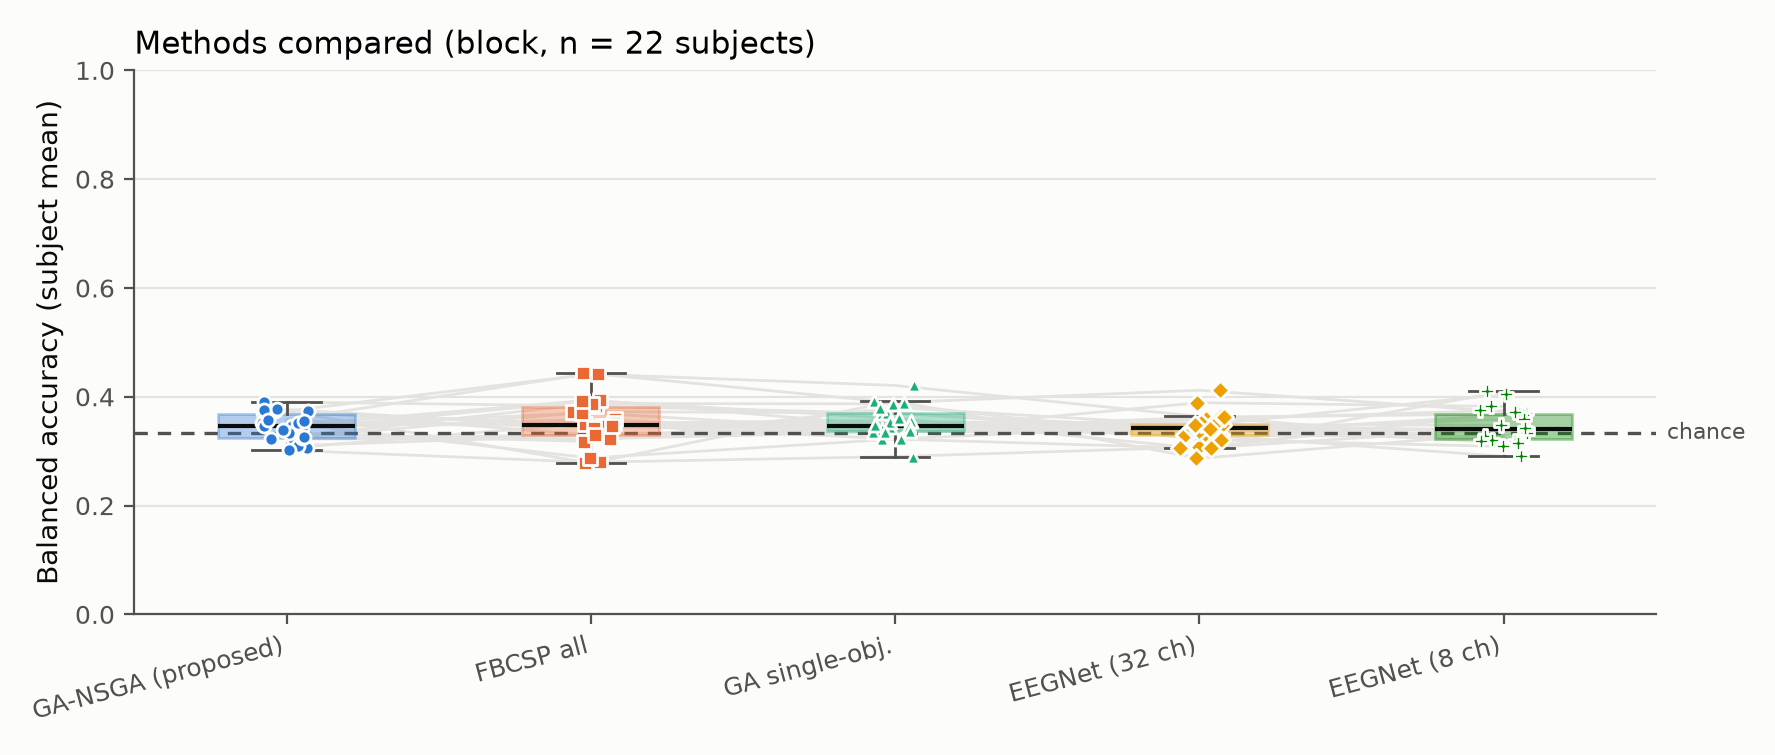
\includegraphics[width=0.92\linewidth]{F01_method_comparison_block.png}
\caption{Subject-level balanced accuracy, block protocol ($n=22$). One dot per subject; the dashed line
is chance. The pre-registered primary test is not significant.}
\label{fig:main}
\end{figure}

\begin{figure}[H]
\centering
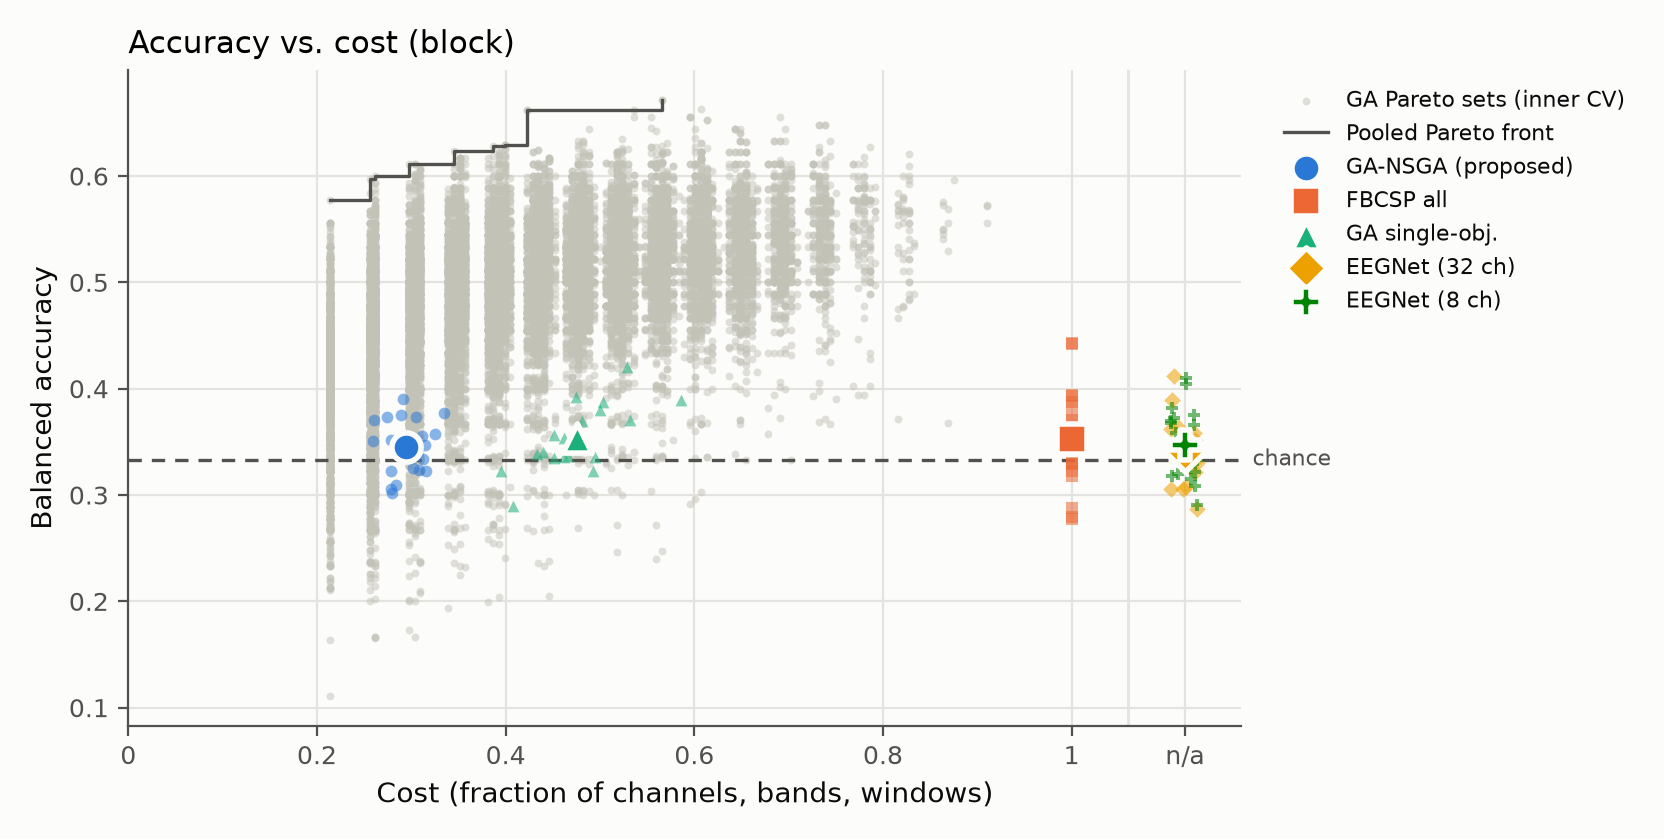
\includegraphics[width=0.80\linewidth]{F02_cost_vs_accuracy_block.png}
\caption{Accuracy against cost (block protocol). Grey points are the GA's inner-CV Pareto entries, which
are optimistic; coloured points are outer-test subject means. \ga\ reaches \fb's accuracy at about
30\,\% of the cost.}
\label{fig:cost}
\end{figure}

\begin{figure}[H]
\centering
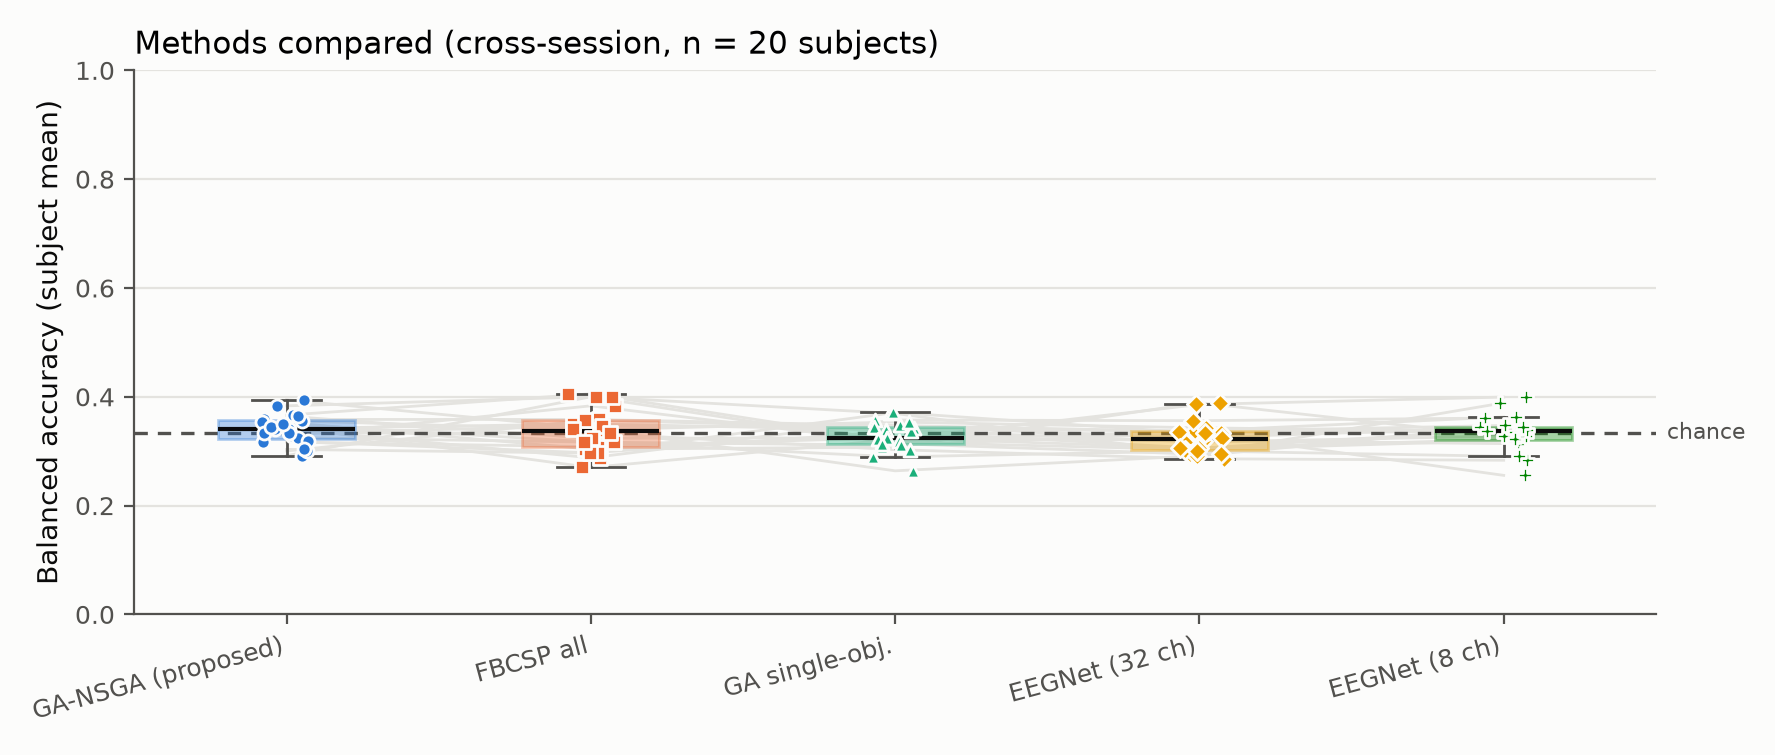
\includegraphics[width=0.85\linewidth]{F03_method_comparison_cross_session.png}
\caption{Cross-session balanced accuracy (train on session 1, test on session 2; $n=20$).}
\label{fig:cross}
\end{figure}

\subsection{What the GA selects}
\ga\ selects on average 2.7 channels, 1.3 bands and 1.6 windows. Selection is nearly flat across genes
(18--43\,\%; most frequent Pz 43\,\%, Oz 38\,\%, P7 35\,\%; Figure~\ref{fig:freq}). Selection stability
is close to chance and no higher than for the accuracy-only GA (Table~\ref{tab:stab}).

\begin{table}[H]
\centering\small
\caption{Selection and stability of the chosen chromosomes (block protocol; Kuncheva index, mean over
recordings).}
\label{tab:stab}
\begin{tabular}{@{}lcccc@{}}
\toprule
Method & Ch / bands / windows & KI (all pairs) & KI (same fold, other seed) & KI (same seed, other fold) \\
\midrule
\ga & 2.7 / 1.3 / 1.6 & 0.078 & 0.163 & 0.072 \\
\gas & 3.8 / 2.0 / 3.2 & 0.084 & 0.254 & 0.058 \\
\bottomrule
\end{tabular}
\end{table}

\begin{figure}[H]
\centering
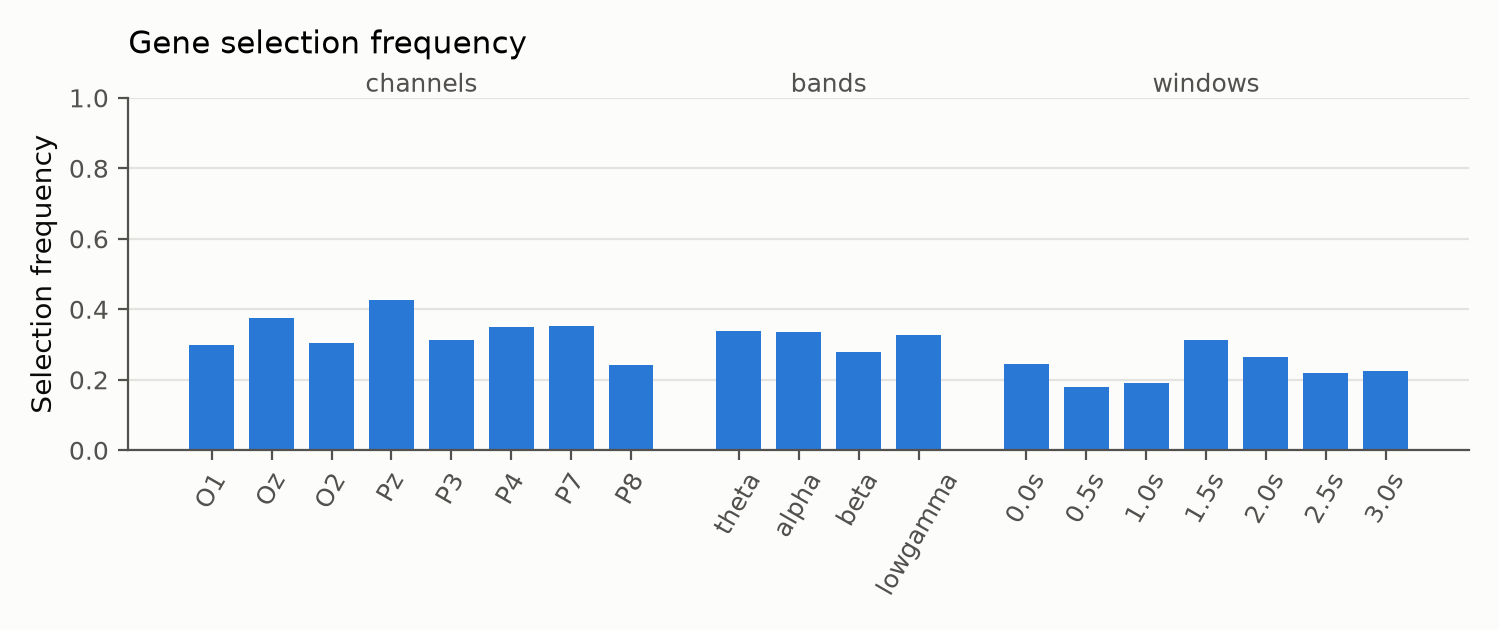
\includegraphics[width=0.78\linewidth]{F04_selection_frequency_ga_nsga.png}
\caption{How often \ga\ selects each gene (504 chosen chromosomes: 126 block runs $\times$ 4 folds).
The near-flat profile shows no consistent preference.}
\label{fig:freq}
\end{figure}

% ------------------------------------------------------------------ 7
\section{Exploratory Analyses}\label{sec:explore}
The following checks were \emph{not} part of the analysis plan. They test why the GA does not help.

\subsection{Random chromosomes at matched cost}
For every outer fold, 50 random chromosomes with exactly the same numbers of channels, bands and windows
as the GA's choice were scored on the same test fold with the same classifier.
\begin{itemize}
  \item \ga\ vs random: $+0.004$ ($p=0.42$); \gas\ vs random: $+0.007$ ($p=0.20$).
  \item The GA's mean percentile among the random draws is 0.51 / 0.52 (0.5 = a typical random subset).
  \item Random subsets at 30\,\% of the cost lose only 0.011 against \fb\ (n.s.).
\end{itemize}
\textbf{The GA search adds nothing beyond the cost reduction} (Figure~\ref{fig:random}).

\begin{figure}[H]
\centering
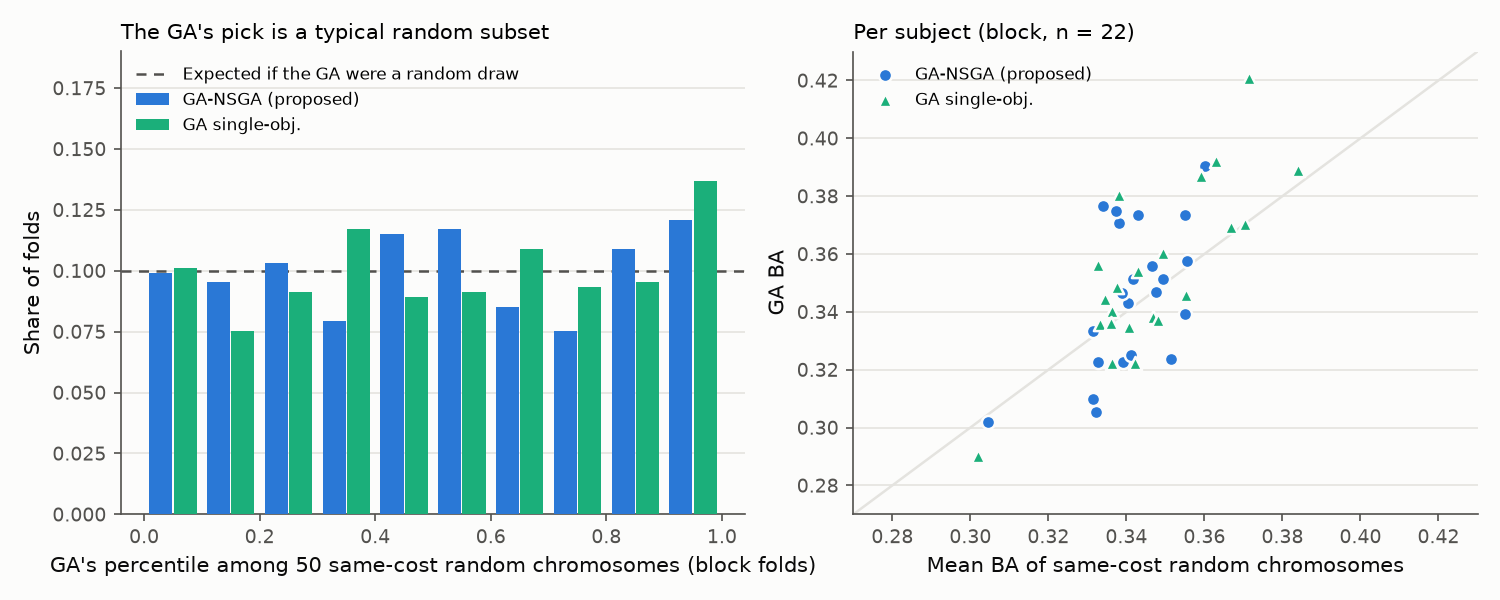
\includegraphics[width=\linewidth]{F06_random_control.png}
\caption{Left: the GA's percentile among 50 same-cost random chromosomes per fold; the flat histogram
means its pick is a typical random subset. Right: per subject, GA accuracy vs the mean accuracy of the
random subsets.}
\label{fig:random}
\end{figure}

\subsection{Alternative chooser rules}
Seven rules were applied to the stored GA fronts: best inner accuracy, 0.5/1/2\,SD, standard error, knee
point and minimum cost. They give 0.338--0.351 on the block protocol. None differs from the contract rule
or from \fb\ (all $p\ge0.28$; Figure~\ref{fig:chooser}). These are test-set scores, so choosing a rule by
them would be selection on the test set.

\begin{figure}[H]
\centering
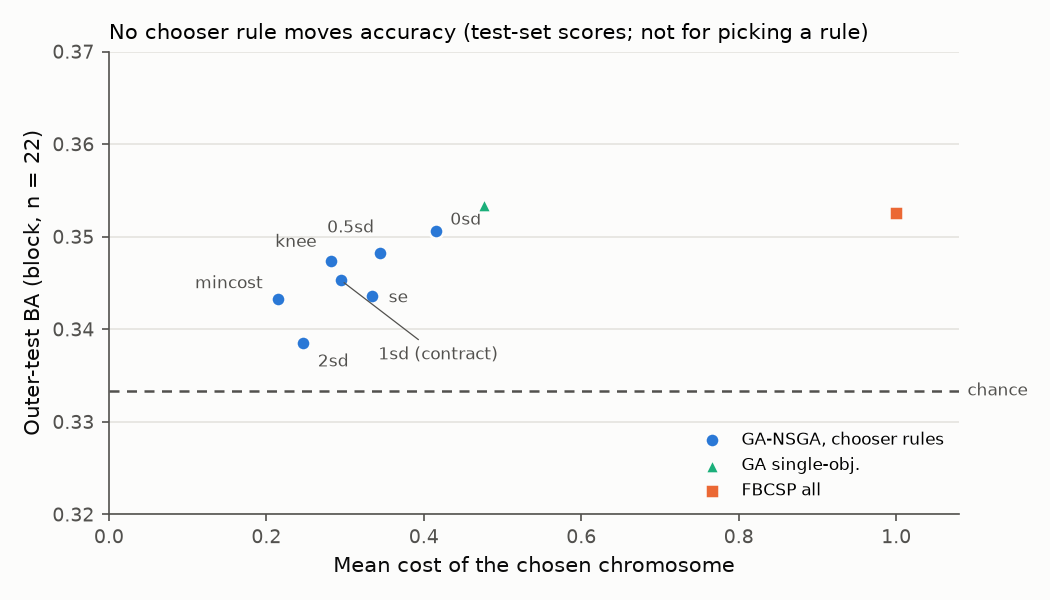
\includegraphics[width=0.78\linewidth]{F07_chooser_rules_block.png}
\caption{Outer-test accuracy against cost for alternative chooser rules on the stored \ga\ fronts.}
\label{fig:chooser}
\end{figure}

\subsection{Training versus test accuracy}
Each fold's classifier was refitted on its outer training set and also scored on those training trials
(Table~\ref{tab:train}, Figure~\ref{fig:train}). EEGNet trained for 300 epochs without early stopping
reaches a training accuracy of 1.0 while its validation accuracy stays at chance (Figure~\ref{fig:curves}).

\begin{table}[H]
\centering\small
\caption{Training, inner-CV and test balanced accuracy (block protocol). For EEGNet the middle column is
the validation accuracy.}
\label{tab:train}
\begin{tabular}{@{}lccc@{}}
\toprule
Method & Training BA & Inner-CV / validation BA & Test BA \\
\midrule
\fb & 0.999 & 0.342 & 0.353 \\
\gas & 0.751 & 0.568 & 0.353 \\
\ga & 0.576 & 0.512 & 0.345 \\
EEGNet (32 ch, P4 recipe) & 0.639 & 0.364 & 0.350 \\
EEGNet (32 ch, 300 epochs, no early stopping) & 1.000 & 0.335 & 0.327 \\
\bottomrule
\end{tabular}
\end{table}

\begin{figure}[H]
\centering
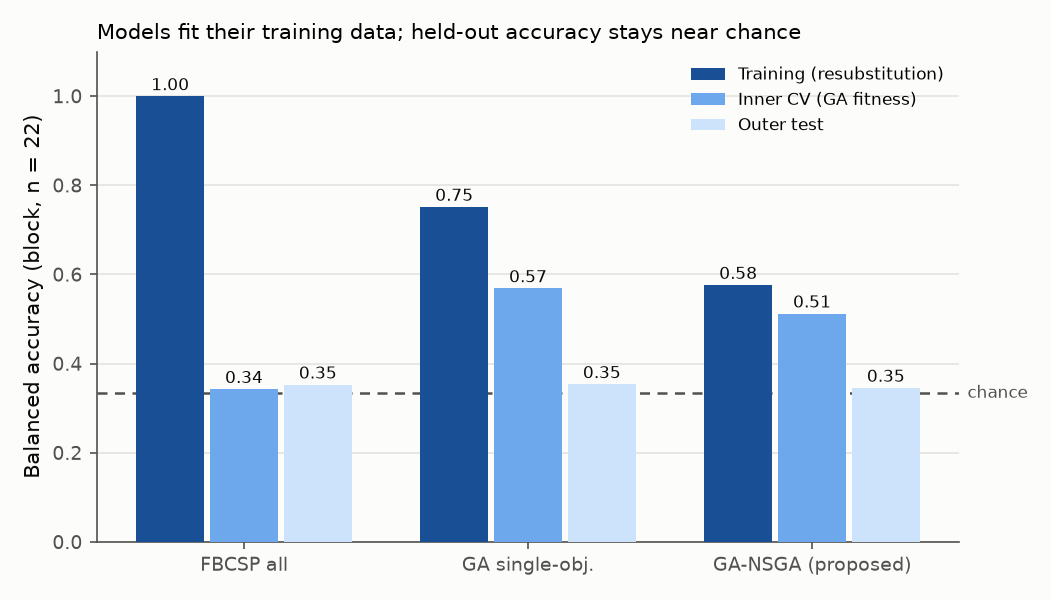
\includegraphics[width=0.66\linewidth]{F05_train_inner_test.png}
\caption{Training vs inner-CV vs test balanced accuracy (block protocol). Every model fits its training
trials but generalises to about chance~$+0.02$; the GA's inner-CV score is inflated by selection.}
\label{fig:train}
\end{figure}

\begin{figure}[H]
\centering
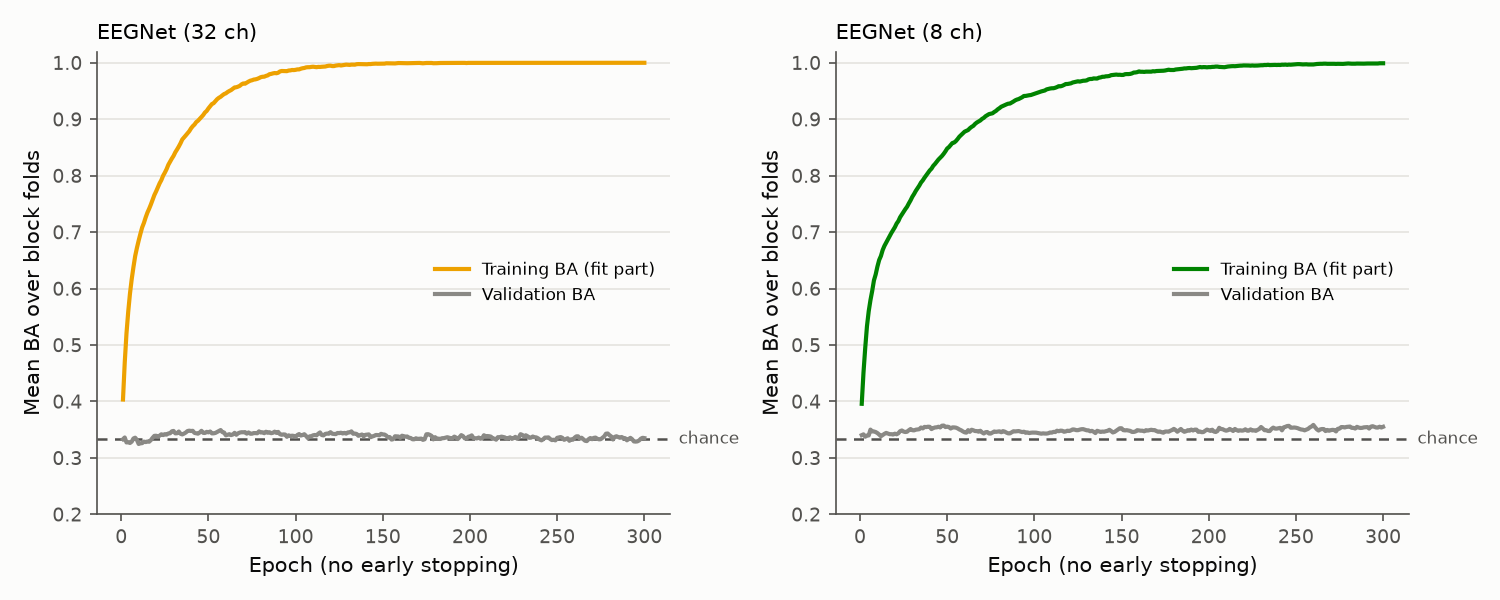
\includegraphics[width=\linewidth]{F10_eegnet_learning_curves.png}
\caption{EEGNet learning curves without early stopping (300 epochs, block folds, seed 0): training
accuracy reaches 1.0 while validation accuracy stays at chance.}
\label{fig:curves}
\end{figure}

\subsection{Trial-position confound}\label{sec:position}
A classifier that sees only the trial's position within its block, with no EEG, predicts the class
across sessions at 0.397 ($p<0.001$; 0.390 without subject 01). The reason is that 30-trial block
orders recur across sessions for 10 of 20 subjects. The EEG methods do not follow this signal: they show
no gain on the shared-block subjects (\fb\ 0.337 vs 0.337) and trial-level agreement $\kappa\approx0$
(Figure~\ref{fig:position}). For subject 01, position and class are perfectly confounded, so its
cross-session result cannot be interpreted.

\begin{figure}[H]
\centering
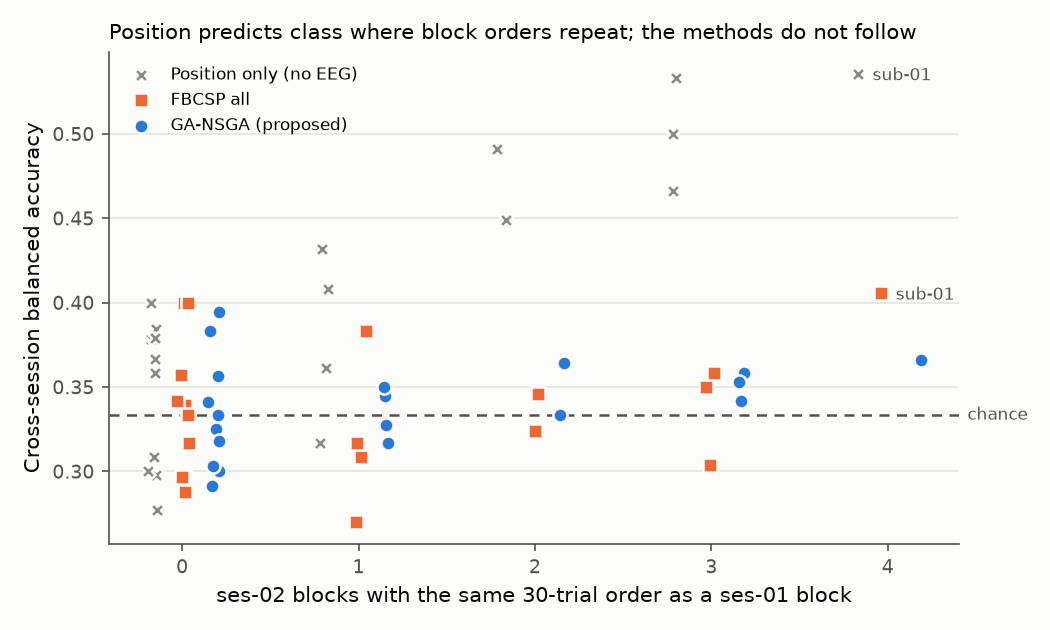
\includegraphics[width=0.78\linewidth]{F08_position_control_cross_session.png}
\caption{Position-only control (cross-session) against the number of session-2 blocks whose order also
occurs in session 1.}
\label{fig:position}
\end{figure}

\subsection{Random-split inflation}
Random stratified 5-fold splits mix temporally adjacent trials into training and test, which can let slow
drifts look predictive. Here they do not inflate any method: the change from block to random splits is
$-0.002$ to $-0.011$ (all n.s.; Figure~\ref{fig:drift}).

\begin{figure}[H]
\centering
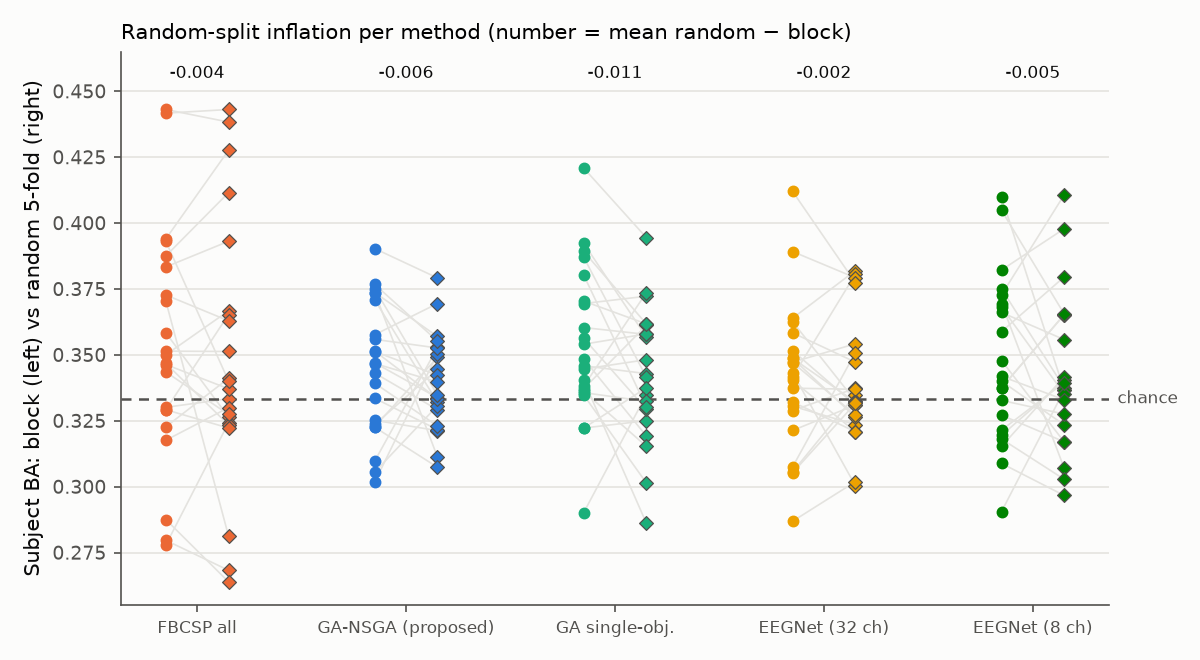
\includegraphics[width=0.85\linewidth]{F09_random_vs_block.png}
\caption{Subject accuracy under leave-one-block-out (left) and random 5-fold splits (right).}
\label{fig:drift}
\end{figure}

\subsection{Perception (viewing) period}
On the 3--7\,s viewing period, where the participant sees the shape, all methods decode well above the
imagery period (Table~\ref{tab:view}, Figure~\ref{fig:view}). Here \ga\ is significantly worse than \fb\
($-0.025$, $p=0.004$) and than \gas\ ($-0.018$, $p=0.04$), and the chooser rule matters (0.377--0.421
across rules).

\begin{table}[H]
\centering\small
\caption{Viewing period vs imagery (block protocol, $n=22$).}
\label{tab:view}
\begin{tabular}{@{}lccccc@{}}
\toprule
Method & Imagery BA & Viewing BA & Difference & $p$ & Recordings $>$ chance (Holm) \\
\midrule
\fb & 0.353 & $0.435\pm0.069$ & $+0.083$ & $<0.001$ & 12/42 \\
\gas & 0.353 & $0.428\pm0.074$ & $+0.074$ & $<0.001$ & 20/42 \\
\ga & 0.345 & $0.410\pm0.048$ & $+0.065$ & $<0.001$ & 15/42 \\
\bottomrule
\end{tabular}
\end{table}

\begin{figure}[H]
\centering
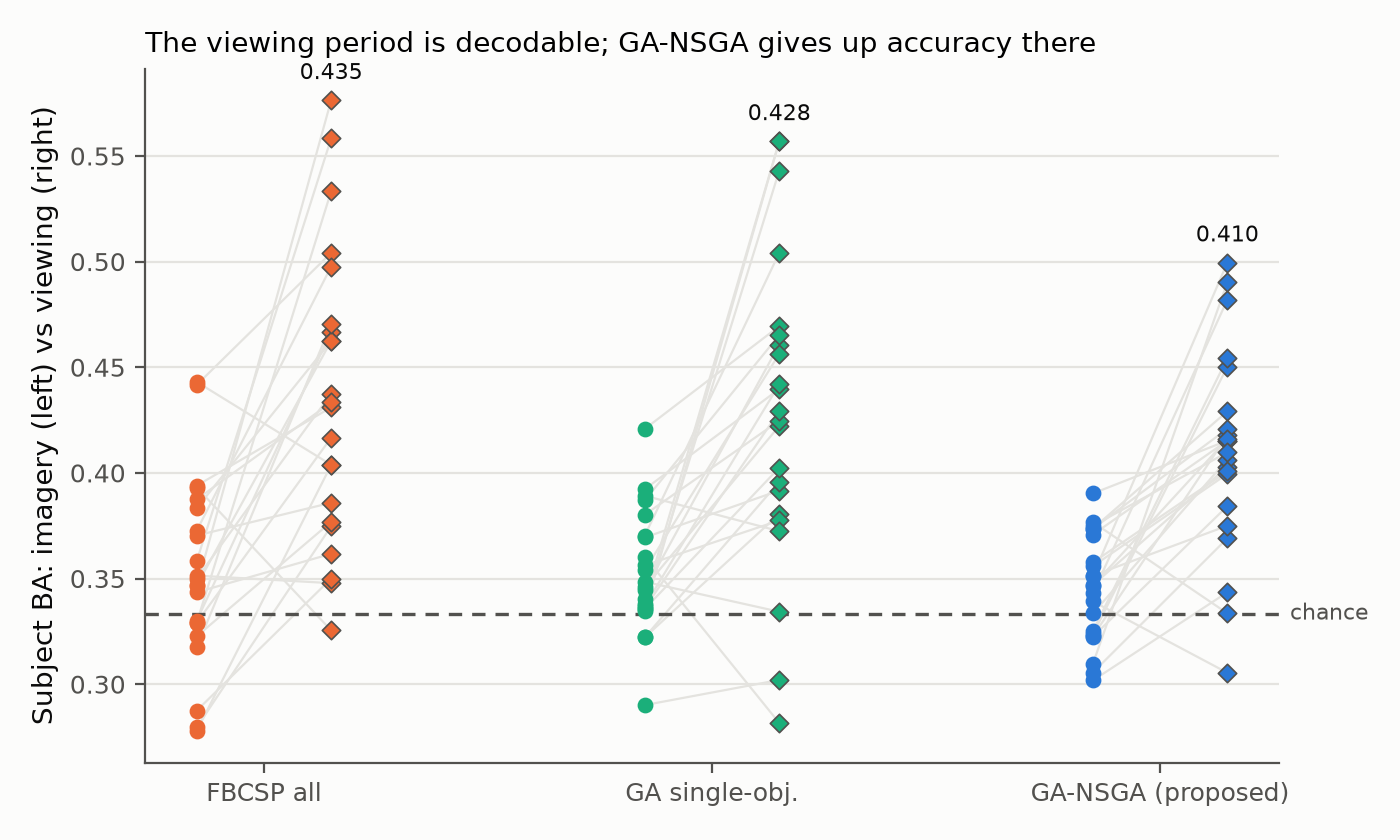
\includegraphics[width=0.78\linewidth]{F11_viewing_vs_imagery.png}
\caption{Imagery (left) vs viewing (right) per subject. With a real signal, the GA's cost pressure costs
accuracy.}
\label{fig:view}
\end{figure}

% ------------------------------------------------------------------ 8
\section{Discussion}

\paragraph{The overfitting gap.} Every model fits its training trials, from 0.58 training accuracy
(\ga, 13 features) to 1.00 (\fb\ with 168 features, and EEGNet without early stopping), yet all land at
about 0.35 on unseen trials. Shrinking the model to 13 features lowers the training fit but not the test
accuracy. The limiting factor is the information in the imagery EEG, not the classifier.

\paragraph{Why the GA cannot help.} The GA's fitness is a 3-fold inner CV on about 90 trials, which is
dominated by noise~\cite{varoquaux2018}. Without selection this estimate is honest: \fb's inner CV is
0.342 against a test accuracy of 0.353. The GA takes the best of about 600 such estimates per fold and
therefore selects lucky chromosomes. This is the \emph{winner's curse} of model
selection~\cite{cawley2010}, and it inflates the inner accuracy by $+0.17$ (\ga) and $+0.21$ (\gas). The
stability objective $\sigma_{in}$ comes from the same three folds and is equally noisy, so it does not
make the selection reproducible (KI 0.08). Selection can only help when some components carry more class
information than others \emph{and} the inner CV can detect it; on the imagery data neither holds.

\paragraph{When there is a signal.} On the viewing period the expected trade-off appears: smaller models
lose accuracy, and the GA's cost pressure costs 0.025 BA for a 67\,\% cost reduction. The stability-aware
GA is therefore a \emph{cost-reduction} tool with a measurable price, not a way to recover a weak signal.

\paragraph{Comparison with the literature.} Gao et al.~\cite{gao2026} report 75.1\,\% for EEGNet on these
three figure classes with a within-subject protocol. Under our pipeline EEGNet reaches 0.341 (block) and
0.339 with random 5-fold splits, which the dataset notes identify as the authors' protocol, so split
leakage does not explain the difference. Differences in epoching, preprocessing or training details remain
possible. We could not reproduce the published figure, and reconciling the two pipelines is future work.
The literature values in Table~\ref{tab:lit} come from different datasets, classes and protocols and are
not directly comparable.

% ------------------------------------------------------------------ 9
\section{Limitations}
\begin{itemize}
  \item \textbf{Class set:} three classes (circle, square, pentagram) instead of the proposal's four,
        because no public dataset contains triangle and hexagon in this paradigm.
  \item \textbf{Weak signal and sample size:} group accuracy is at most 0.02 above chance; with $n=22$
        only differences of about 0.024 BA or more are detectable.
  \item \textbf{Fixed design:} the candidate channels, bands, windows, GA budget (30$\times$20) and
        EEGNet recipe were frozen before the results; other search spaces were not tried.
  \item \textbf{Small inner CV:} three folds of about 30 trials are the GA's only fitness signal.
  \item \textbf{Trial-order confounds} in the dataset (Section~\ref{sec:position}) affect any
        cross-session or cross-subject analysis.
  \item \textbf{Artefact handling} uses the 8 candidate channels only (no EOG or ICA), so 32-channel
        EEGNet sees frontal blink activity.
  \item \textbf{Exploratory analyses} were not corrected for multiplicity across checks.
\end{itemize}

% ------------------------------------------------------------------ 10
\section{Conclusion and Future Work}
On 22 subjects, a stability-aware NSGA-II that jointly selects EEG channels, frequency bands and time
windows \textbf{did not outperform} filter-bank CSP on all components for imagined-shape decoding (0.345
vs 0.353 balanced accuracy, $p=0.79$). It also did not outperform an accuracy-only GA or EEGNet. It
delivers the same near-chance accuracy at about 30\,\% of the cost, but its selections are no better than
random subsets of the same size and are not reproducible. Every model memorises its training data and
generalises to about chance~$+0.02$, so the imagery signal of this dataset, not the classifier, is the
bottleneck. When a real signal exists (the perception period), the GA's cost reduction has a significant
accuracy price.

\paragraph{Future work.}
\begin{itemize}
  \item Evaluate the method on a dataset with the proposal's four shapes (circle, square, triangle,
        hexagon) and more trials per class.
  \item Reconcile our EEGNet pipeline with the 75.1\,\% reported by Gao et al.
  \item Use fitness estimates that are robust to the winner's curse (repeated inner CV, nested
        stability selection) or multi-session training.
  \item Apply the selection where a signal is strong (perception, or imagery with feedback training) and
        the cost of channels matters, e.g.\ low-channel wearable BCIs.
\end{itemize}

% ------------------------------------------------------------------ appendix
\appendix
\section{Reproducibility and Software}
\begin{itemize}
  \item \textbf{Code:} Python package with fixed module contracts (\texttt{src/}: io, preprocess, cv,
        fbcsp, ga, eegnet, analysis), 200 automated tests, and release tag \texttt{v1.0}.
  \item \textbf{Determinism:} GA results are bit-identical across the three team machines, and EEGNet is
        deterministic on CUDA. Every result file records its code commit, configuration hash
        (\texttt{08e124167b}) and host.
  \item \textbf{Pre-registration and deviations:} the analysis plan was pushed before the group results
        were analysed. One machine had run the grid locally before the plan was pushed; those files were
        never used, and the official runs are bit-identical to them. All deviations are documented.
  \item \textbf{Run times} (i5-13450HX, RTX 3050 6\,GB): cache build $\approx$7\,min, baseline 9\,s,
        full GA grid 5.3\,min, EEGNet 49\,min.
\end{itemize}

\section{Team Contributions}
\begin{tabularx}{\linewidth}{@{}lY@{}}
\toprule
Member & Responsibilities \\
\midrule
Abhay Nagesh Rao (26CSM1R01) & Cross-validation splits, FBCSP + shrinkage LDA, statistical analysis and figures; GA runs for subjects 09--16. \\
Pandya Aditya Deepakkumar (26CSM1R02) & Data download, BIDS reading, preprocessing and caches, integration, FBCSP baseline, pre-registered analysis plan; GA runs for subjects 01--08. \\
Mulakalapalli Jayachandra Siddhartha (26CSM1R07) & Genetic algorithms (NSGA-II, single-objective), EEGNet, GA runs for subjects 17--22 and all EEGNet runs, exploratory analyses, final results and release. \\
\bottomrule
\end{tabularx}

% ------------------------------------------------------------------ references
\begin{thebibliography}{99}\small
\bibitem{esfahani2012} E.~T. Esfahani and V.~Sundararajan, ``Classification of primitive shapes using
brain--computer interfaces,'' \emph{Computer-Aided Design}, vol.~44, no.~10, pp.~1011--1019, 2012.
doi: 10.1016/j.cad.2011.04.008.
\bibitem{costa2019} F.~R. Llorella Costa, G.~Patow, and J.~M. Azor\'{\i}n, ``Common spatial pattern for the
classification of imagined geometric objects,'' in \emph{Proc. 3rd Int. Conf. Computer-Human Interaction
Research and Applications (CHIRA)}, pp.~152--155, 2019. doi: 10.5220/0007934601520155.
\bibitem{llorella2020} F.~R. Llorella, G.~Patow, and J.~M. Azor\'{\i}n, ``Convolutional neural networks and
genetic algorithm for visual imagery classification,'' \emph{Physical and Engineering Sciences in
Medicine}, vol.~43, no.~3, pp.~973--983, 2020. doi: 10.1007/s13246-020-00894-z.
\bibitem{llorella2021} F.~R. Llorella, E.~I\'a\~nez, J.~M. Azor\'{\i}n, and G.~Patow, ``Classification of
imagined geometric shapes using EEG signals and convolutional neural networks,'' \emph{Neuroscience
Informatics}, vol.~1, no.~4, art.~100029, 2021. doi: 10.1016/j.neuri.2021.100029.
\bibitem{korik2024} A.~Korik, N.~du~Bois, G.~Campbell, E.~O'Neill, L.~Hay, S.~Gilbert, M.~Grealy, and
D.~Coyle, ``Real-time feedback improves imagined 3D primitive object classification from EEG,''
\emph{Brain-Computer Interfaces}, vol.~11, nos.~1--2, pp.~61--85, 2024. doi: 10.1080/2326263X.2024.2334558.
\bibitem{gao2026} J.~Gao, Y.~Liu, Z.~Li, K.~Huang, F.~Wang, J.~Xu, L.~Zhao, T.~Li, and Y.~Fu, ``An EEG
dataset for visual imagery-based brain--computer interface,'' \emph{Scientific Data}, vol.~13, art.~194,
2026. doi: 10.1038/s41597-025-06512-5.
\bibitem{ang2008} K.~K. Ang, Z.~Y. Chin, H.~Zhang, and C.~Guan, ``Filter bank common spatial pattern (FBCSP)
in brain-computer interface,'' in \emph{Proc. IEEE Int. Joint Conf. Neural Networks (IJCNN)},
pp.~2390--2397, 2008.
\bibitem{deb2002} K.~Deb, A.~Pratap, S.~Agarwal, and T.~Meyarivan, ``A fast and elitist multiobjective
genetic algorithm: NSGA-II,'' \emph{IEEE Trans. Evolutionary Computation}, vol.~6, no.~2, pp.~182--197, 2002.
\bibitem{pymoo} J.~Blank and K.~Deb, ``pymoo: Multi-objective optimization in Python,'' \emph{IEEE Access},
vol.~8, pp.~89497--89509, 2020.
\bibitem{ledoit2004} O.~Ledoit and M.~Wolf, ``A well-conditioned estimator for large-dimensional covariance
matrices,'' \emph{J. Multivariate Analysis}, vol.~88, no.~2, pp.~365--411, 2004.
\bibitem{lawhern2018} V.~J. Lawhern, A.~J. Solon, N.~R. Waytowich, S.~M. Gordon, C.~P. Hung, and B.~J.
Lance, ``EEGNet: a compact convolutional neural network for EEG-based brain--computer interfaces,''
\emph{J. Neural Engineering}, vol.~15, no.~5, art.~056013, 2018.
\bibitem{schirrmeister2017} R.~T. Schirrmeister et al., ``Deep learning with convolutional neural networks
for EEG decoding and visualization,'' \emph{Human Brain Mapping}, vol.~38, no.~11, pp.~5391--5420, 2017.
\bibitem{kuncheva2007} L.~I. Kuncheva, ``A stability index for feature selection,'' in \emph{Proc. 25th
IASTED Int. Multi-Conference: Artificial Intelligence and Applications}, pp.~390--395, 2007.
\bibitem{wilcoxon1945} F.~Wilcoxon, ``Individual comparisons by ranking methods,'' \emph{Biometrics
Bulletin}, vol.~1, no.~6, pp.~80--83, 1945.
\bibitem{holm1979} S.~Holm, ``A simple sequentially rejective multiple test procedure,'' \emph{Scandinavian
J. Statistics}, vol.~6, no.~2, pp.~65--70, 1979.
\bibitem{varoquaux2018} G.~Varoquaux, ``Cross-validation failure: small sample sizes lead to large error
bars,'' \emph{NeuroImage}, vol.~180, pp.~68--77, 2018.
\bibitem{cawley2010} G.~C. Cawley and N.~L.~C. Talbot, ``On over-fitting in model selection and subsequent
selection bias in performance evaluation,'' \emph{J. Machine Learning Research}, vol.~11, pp.~2079--2107,
2010.
\end{thebibliography}

\end{document}
